\documentclass[12pt]{article}
\usepackage{titlesec}
\usepackage{subcaption}
\usepackage[scaled]{helvet}  \renewcommand\familydefault{\sfdefault} % Font
\usepackage{graphicx} % Required for inserting images
\usepackage{geometry}
\usepackage{pgfplotstable}
\usepackage{amsmath}
\usepackage{enumitem}
\usepackage{tikz} 
\usetikzlibrary{petri,arrows.meta}
\geometry{a4paper, total={170mm,257mm},left=20mm, top=20mm,}
\usepackage[listings,breakable,skins]{tcolorbox}
% declare our code block environment
  \newtcblisting{tcbcodeblock}[1]{%
    enhanced,
    sharp corners,
    colframe=black,
    coltext=codefg,
    colback=codebg,
    breakable,
    size=fbox,
    listing only,
    listing options={%
      style=tcblatex,
      language={#1},
      showspaces=false,
      showstringspaces=false,
      commentstyle=\color{codegray},
      keywordstyle=\color{codegreen},
      stringstyle=\color{codecyan},
      basicstyle=\ttfamily\footnotesize
    }
  }
\renewcommand{\thesection}{\Roman{section}}
\renewcommand{\thesubsection}{\arabic{subsection}}
\renewcommand{\thesubsubsection}{\alph{subsubsection}.}

\titleformat{\section}{\normalfont\LARGE\bfseries}{\thesection.}{10pt}{}
\titleformat{\subsection}{\normalfont\Large}{\thesubsection.}{10pt}{}
\titleformat{\subsubsection}{\normalfont\large}{\thesubsubsection}{10pt}{}

\begin{document}
\thispagestyle{empty} %Suppress number of this page
\begin{center}
    \vspace{7pt}
    \fontsize{18pt}{17pt}\selectfont 
    \textbf{University of Science and Technology of Hanoi}
    \vspace{7pt}
\end{center}

\vspace{90pt}

\begin{center}
    \fontsize{30pt}{17pt}\selectfont 
    \textbf{Deep learning} 
    \vspace{50pt}

    \fontsize{20pt}{17pt}\selectfont 
    \textbf{Labwork 1}
    \vspace{50pt}


    \fontsize{17pt}{17pt}\selectfont
    \textbf{{Student id: }{2440057}}
    \vspace{15pt}

    \fontsize{17pt}{17pt}\selectfont
    \textbf{{Student name: }{Nguyen Nhat Anh}}
    \vspace{15pt}
    
\end{center}

\newpage
\setcounter{page}{1} % Start number from this page
\section{How I Implemented the Algorithm}
In this lab, I implemented Gradient Descent from scratch in Python without using any external libraries.

We aim to minimize the function:
\[
f(x) = x^2, \quad \text{with derivative} \quad f'(x) = 2x
\]

We start with an initial value of \( x \) and iteratively apply the update rule:
\[
x_{t+1} = x_t - r \cdot f'(x_t)
\]
Where:
\begin{itemize}
  \item \( r \) is the learning rate
  \item \( f'(x_t) = 2x_t \) is the gradient at current \( x \)
\end{itemize}
\\
Below is the Python implementation:
\begin{verbatim}
def minimize_quadratic(x, lr):
    history = []

    while x > 0.1:
        loss = x * x
        history.append(loss)
        print(f"Current loss: {loss:.4f}")
        x -= lr * 2 * x

    return history

loss_values = minimize_quadratic(10, 0.1)
\end{verbatim}

\section{{Implement with learning rate = 0.1}}
\subsection{Learning rate = 0.1}
\begin{center}
\begin{tabular}{|c|c|c|}
\hline
Iteration & $x$ & $f(x)$ \\
\hline
0 & 10.0000 & 100.0000 \\
1 & 8.0000 & 64.0000 \\
2 & 6.4000 & 40.9600 \\
3 & 5.1200 & 26.2144 \\
4 & 4.0960 & 16.7772 \\
5 & 3.2768 & 10.7374 \\
6 & 2.6214 & 6.8719 \\
7 & 2.0972 & 4.4020 \\
8 & 1.6777 & 2.8133 \\
9 & 1.3422 & 1.8005 \\
\hline
\end{tabular}
\end{center}

\begin{center}
    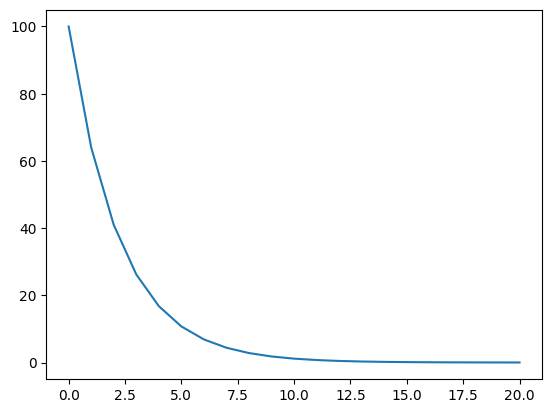
\includegraphics[scale=0.7]{output_0.1.png}
\end{center}

\textbf{Analysis:}
\begin{itemize}
    \item The gradient descent with \( r = 0.1 \) converges much faster than with \( r = 0.01 \).
    \item The updates to \( x \) and \( f(x) \) are more significant in each iteration, and the algorithm reaches values closer to the minimum much more quickly.
    \item By iteration 9, \( x \) has decreased to 1.3422, and \( f(x) \) is 1.8005.
    \item This faster convergence is a result of the larger learning rate, which reduces the function value more rapidly in each step, though there is a slight risk of overshooting the minimum.
\end{itemize}

\subsection{Learning rate = 0.01}
\begin{center}
\begin{tabular}{|c|c|c|}
\hline
Iteration & $x$ & $f(x)$ \\
\hline
0 & 10.0000 & 100.0000 \\
1 & 9.8 & 96.04 \\
2 & 9.604 & 92.2368 \\
3 & 9.41192 & 88.5842 \\
4 & 9.2236816 & 85.0763 \\
5 & 9.039207968000001 & 81.7073 \\
6 & 8.858423808640001 & 78.4717 \\
7 & 8.6812553324672 & 75.3642 \\
8 & 8.507630225817856 & 72.3798 \\
9 & 8.337477621301499 & 69.5135 \\
\hline
\end{tabular}
\end{center}

\begin{center}
    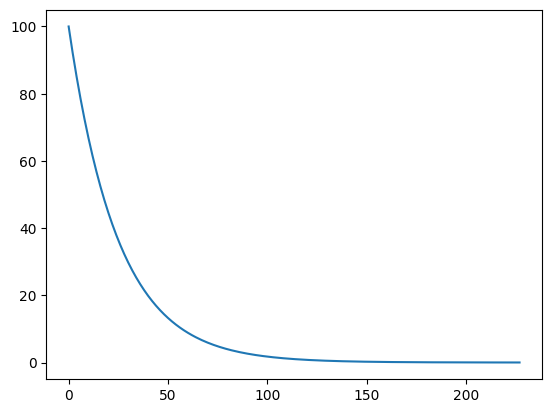
\includegraphics[scale=0.7]{output_0.01.png}
\end{center}

\textbf{Analysis:}
\begin{itemize}
    \item The gradient descent with \( r = 0.01 \) converges slowly. 
    \item Each iteration results in a small decrease in both \( x \) and \( f(x) \).
    \item By iteration 9, \( x \) has decreased to 8.337, and \( f(x) \) is 69.5135, which is still far from the minimum of 0.
    \item The small learning rate results in gradual changes, offering more precise adjustments but requiring more iterations to approach the minimum.
\end{itemize}


\end{document}